\section{Introduction}

Static analysis of code is one of the most effective ways to avoid defects in software, and, when security is a concern, is essential.  Static analysis can find problems that are extremely hard to detect by testing, when the inputs triggering a bug are hard to find.  Static analysis is also often more efficient than testing; a bug that takes a fuzzer days to find may be immediately identified.
Users of static analysis tools often wonder which of multiple tools available for a language are most effective, and how much tools overlap in their results.  Tools often find substantially different bugs, making it important to use multiple tools \cite{AllBugs}.  However, given the high cost of examing results, if a tool provides only marginal novelty, it may not be worth using, especially if it has a high false-positive rate.  Developers of static analysis tools also want to be able to compare their tools to other tools, in order to see what detection patterns or precision/soundness trade-offs they might want to imitate.  Unfortunately, comparing static analysis tools in these ways is hard, and would seem to require vast manual effort to inspect findings and determine ground truth on a scale that would provide statistical confidence.

Differential testing \cite{Differential,ICSEDiff,csmith} is a popular approach to comparing multiple software systems offering similar functionality, but the wide divergence of possible trade-offs, analysis focuses, and the prevalence of false positives in almost all analysis results makes na\"ive differential testing not applicable to static analysis tools \cite{regehrRandom}.
Mutation analysis\cite{jia2011analysis,demillo1978hints,budd1980theoretical} uses small syntactic changes to a program to introduce synthetic ``faults,'' under the assumption that if the original version of a program is mostly correct, such changes will often introduce a fault.  For the most part, mutation analysis has been used to evaluate test suites by computing a mutation score, the fraction of mutants the suite detects, or ``kills''.  
Groce et al. \cite{groce2015verified,groce2018verified} proposed examining individual mutants that survive a rigorous testing and verification effort to detect and correct weaknesses in testing, and found bugs in a heavily-tested module of the Linux kernel \cite{mutKernel} and a widely used Python file system.  Recently, mutation analysis has been adopted in industrial settings, though not for actual examination of all surviving mutants \cite{MutGoogle,ivankovic2018industrial}.

Combining a differential approach and mutation analysis offers a novel way to compare static analysis tools, one useful to users wishing to select a good tool or set of tools, to researchers interested in the impact of precision/soundness trade-offs or different intermediate languages, and to developers of static analysis tools hoping to improve their tools.

%\subsection{Differential Mutation Analysis}

We can say that a static analysis tool kills a mutant when the \emph{number of warnings or errors}, which we call \emph{findings}, \emph{increases with mutation}.  In order to make this definition useful, we ignore informational or optimization related warnings (e.g., if a mutant is merely \emph{stylistically} suboptimal this is not ``finding a fault''). That is, a mutant is killed when a tool ``finds more (unique) bugs'' for the mutated code than for the un-mutated code.  This difference may be most easily interpreted when the original code produces no findings; we call such code \emph{clean} (by analogy with Chekam et al.'s notion \cite{CleanProgram}). For non-clean code, a tool conceivably could detect the mutant, but only change a previously generated finding, not add an additional finding.  However, even for non-clean code, \emph{most detected mutants should produce a new warning}.  We count findings, rather than consider their location or type, because some mutants cause a fault at a far-removed location.  Forcing tools to produce an \emph{additonal} warning is a conservative and automatable estimate of mutant detection.

The value of the differential comparison lies in a few key points.  First, this is a measure that does not reward a tool that produces too many false positives.  The tool cannot simply flag all code as having a problem or it will perform poorly at the task of \emph{distinguishing} the mutated code from non-mutated, and presumably at least \emph{more} correct, code.  Based on verification and testing uses of mutation, it is safe to say that usually at minimum 40\%, often 50-60\%, and frequently up to 80\%+ \cite{mutKernel,groce2018verified,le2014mucheck}, of mutants are not semantically equivalent to the original code \cite{TCE,impactEquiv,smith2009should}, so the task presented to a static analysis tool is simply the core functionality of static analysis: \emph{to distinguish faulty from correct code without execution}.  Obviously, many faults cannot be identified statically without a complete specification, or without unreasonable analysis cost and precision, but the measure of performance here is \emph{relative} to other tools applied to the same code; this is primarily a \emph{differential} approach.  While many mutants cannot be detected statically, the ones that \emph{are} tend to be \emph{true positives}: \emph{if} they were real code changes, they would be faults.  \emph{We manually confirmed that for a large portion of the detected mutants in our experiments, the changes were indeed ones that would be real faults if present in the code.}

Second, and critically, this is an \emph{automatable} method that can provide an evaluation of static analysis tools over a large number of target source code files, without requiring human effort to classify results as real bugs or false positives.  It is not clear that any other fully automatic method is competitively meaningful; it is possible that methods based on code changes from version control provide some of the same benefits, but these require classification of changes into bug-fixes and non-bug-fixes, and of course require version control history.  Also, history-based methods will be biased towards precisely those faults humans or tools already in use were able to detect and fix.  Rather than the hundreds \cite{just2014defects4j} or at most few thousand of faults \cite{BugSwarm} in benchmark defect sets, our approach enables the use of \emph{many tens of thousands} of hypothetical faults.

It is the combination of differential comparison and mutation that is key.  Differential comparison of tools, as noted above, is not really meaningful, without additional effort; na\"ive methods simply will not work \cite{regehrRandom}.  Consider a comparison of the number of findings between two tools over a single program, or over a large set of programs.  If one tool emits more warnings and errors than another, it may mean that the tool is more effective at finding bugs; but it may also mean that it has a higher false positive rate.  Without human examination of the individual findings, it is impossible to be sure.  Using mutants, however, provides a foreground to compare to this background.  In particular, for a large set of programs, the most informative result will be when 1) tool A reports fewer findings on average than tool B over the un-mutated programs but 2) tool A also detects more mutants.  This is strong evidence that A is simply better all-around than B; it likely has a lower false positive rate \emph{and} a lower false negative rate, since it is hard to construct another plausible explanation for reporting \emph{fewer} findings on un-mutated code while still detecting \emph{more} mutants.  Our method (see the \emph{mutant ratio} defined below) provides a quantitative measure of this insight.

\begin{figure}
  \centering
  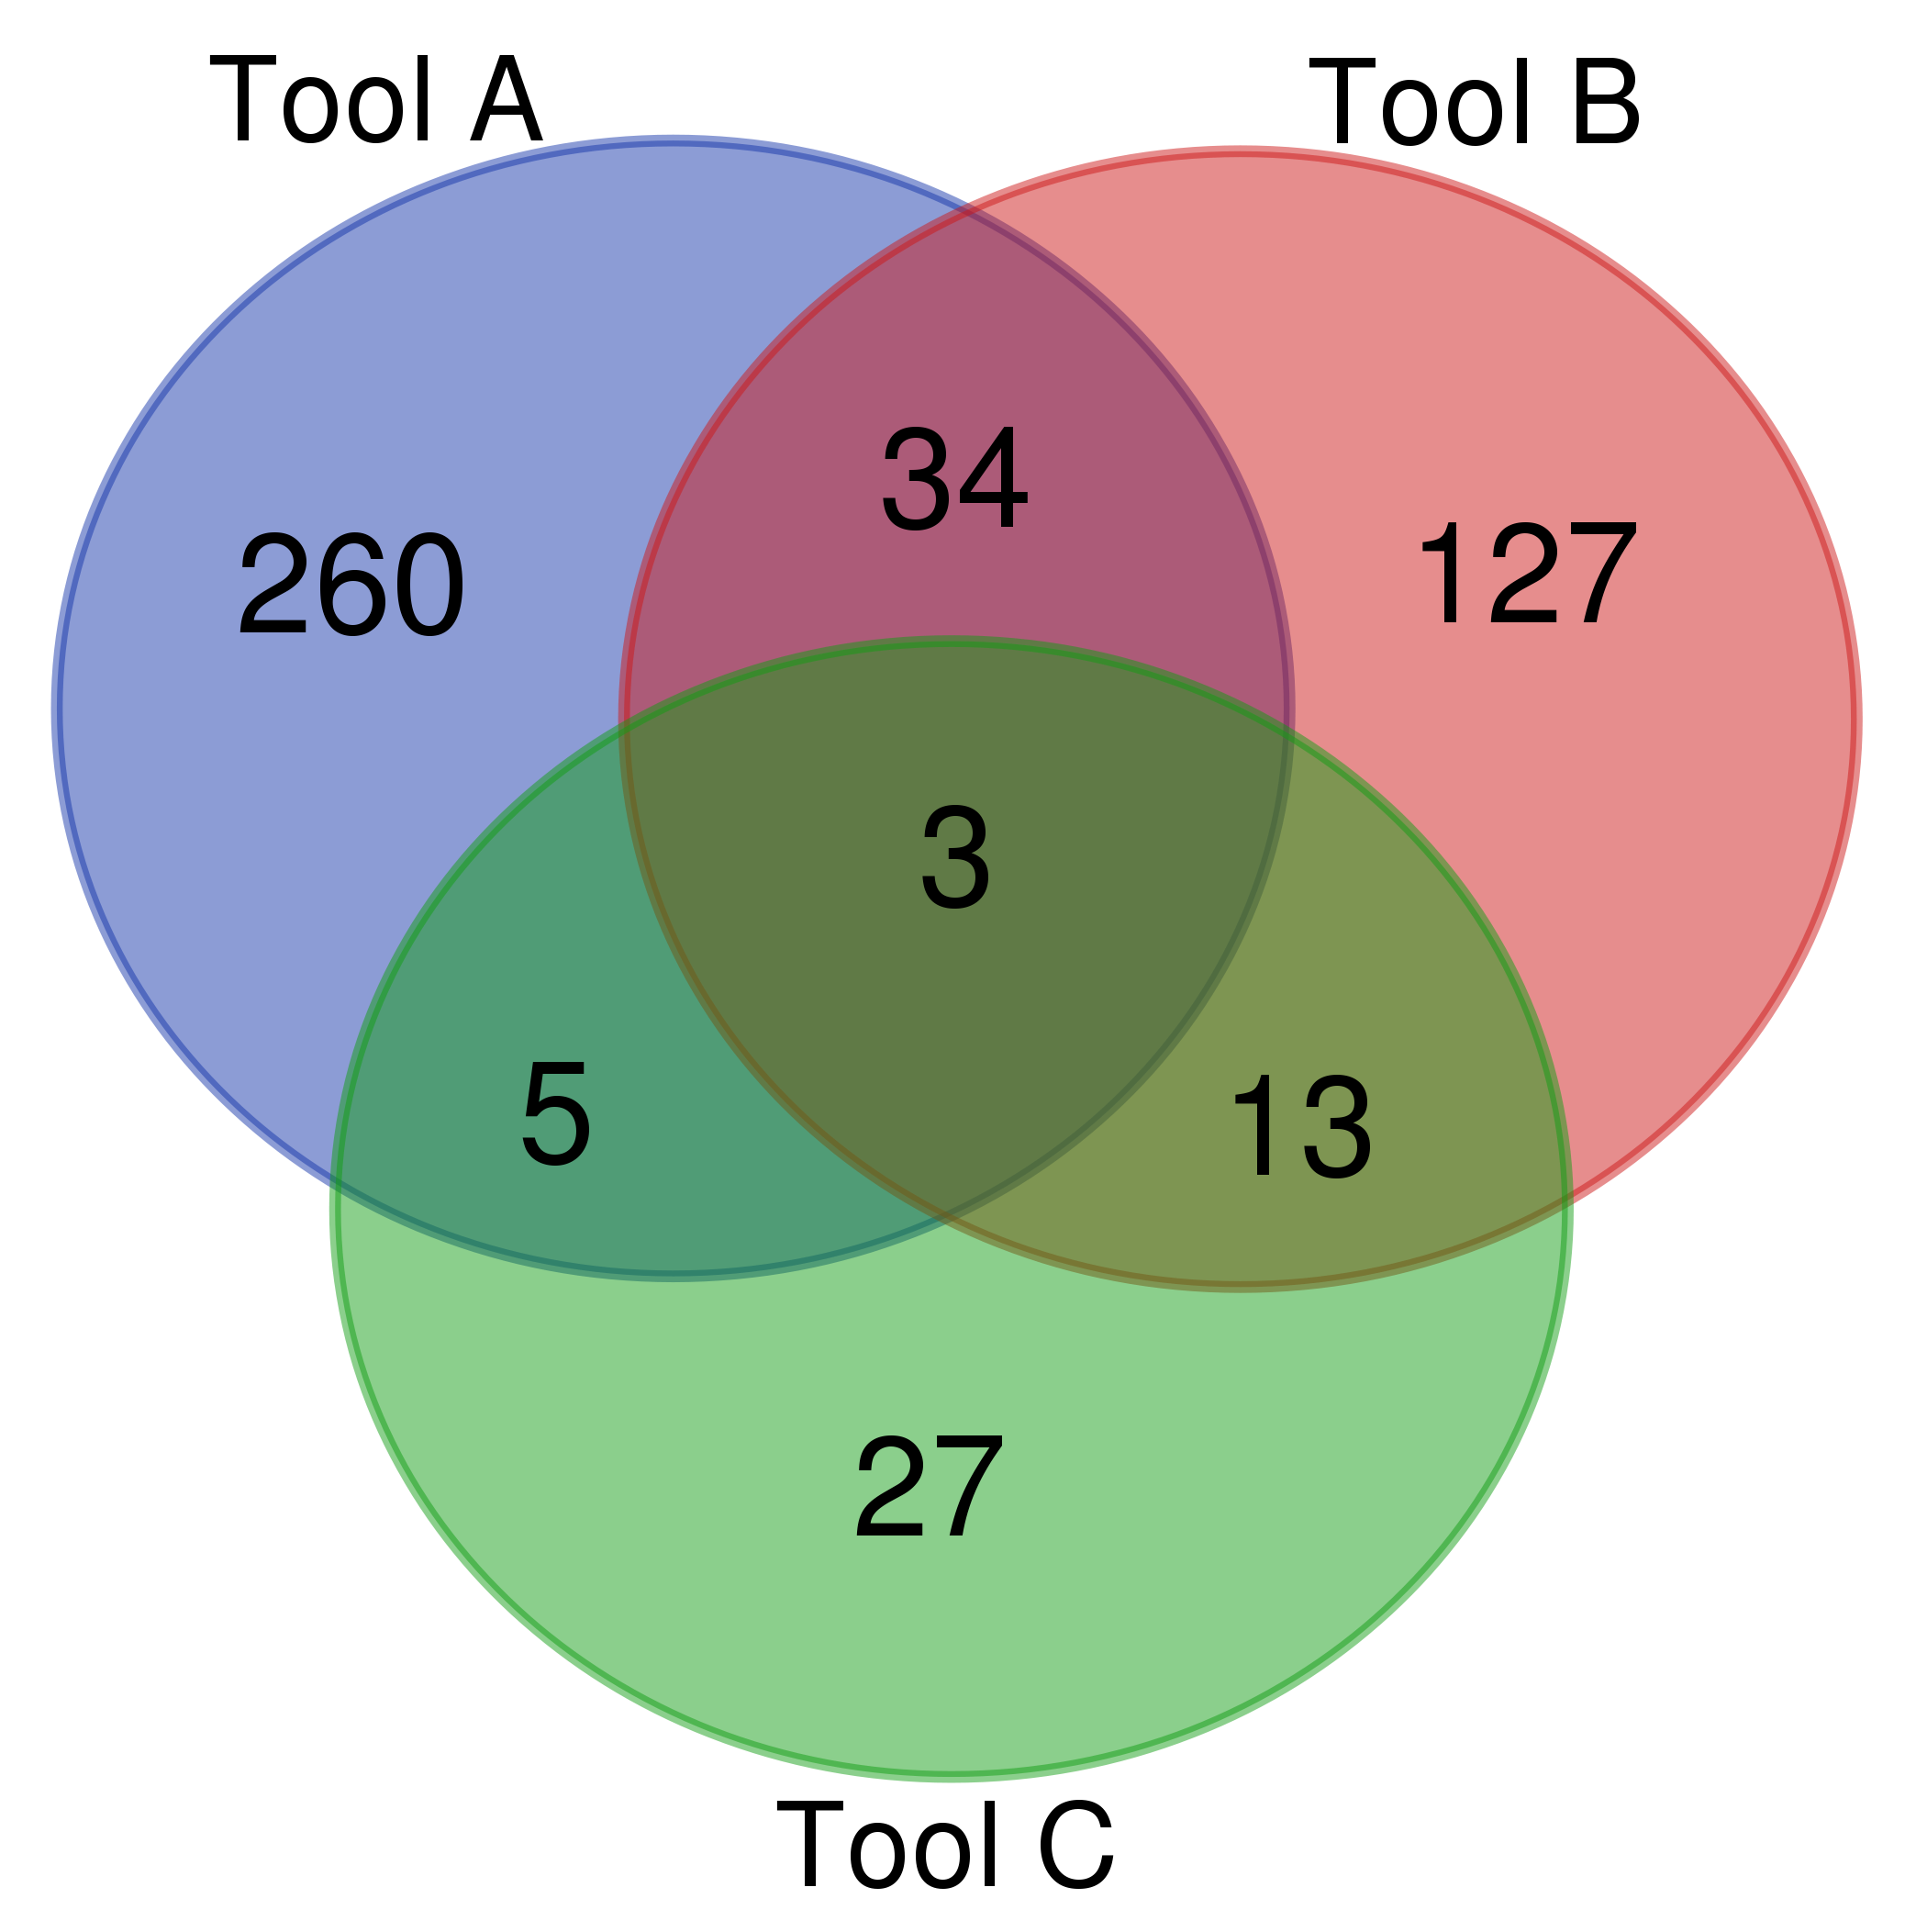
\includegraphics[width=0.30\columnwidth]{example.png}
  \caption{Mutants killed by three static analysis tools.}
  \label{fig:examplevenn}
\end{figure}

Finally, even when tools have similar quantitative results, examining individual mutants killed by one tool but not by another allows us to understand strengths and weaknesses of the tools, in a helpful context: the difference between the un-mutated code and mutated code will always be small and simple.  Moreover, simply looking at how much two tools agree on mutants can answer the question: given that I am using tool A, would adding tool B be likely be worthwhile?  Interested users, e.g. security analysts, can inspect the differences to get an idea of the particular cases when a tool might be most effective, but a more typical user can simply look at a Venn diagram of kills like that shown in Figure \ref{fig:examplevenn}.  Consider hypothetical tools A, B, and C.  A and B produce similar numbers of findings on the code in question, while tool C produces an order of magnitude more findings.  Tool A is likely the most important tool to make use of; it detected more mutants than any other tool, and more than twice as many mutants were killed by A alone than by B alone.  However, also running tool B is well justifed.  B does not do as well as A, but it is the only tool that detects a large number of mutants, and most mutants it detects are unique to it.  Finally, Tool C \emph{may} not be worth running, since its poor performance on mutants but high finding rate suggests it may be prone to missing bugs and to false positives.  It might be a good idea to just look at the 27 mutants detected by C alone:  \emph{if} they represent an important class of potential problems (perhaps C specialized in detecting potentially non-terminating loops), then C might be useful, but if the first few mutants inspected are false positives, then C is likely not useful.

\begin{figure}
{\scriptsize
\begin{code}
contract SimpleStorage \{
    uint storedData;

    function set(uint x) public \{
        storedData = x;
    \}

    function get() public view returns (uint) \{
        return storedData;
    \}
  \}
\end{code}
}
\caption{A simple example Solidity smart contract}
\label{fig:sol424intro}
\end{figure}

More concretely, consider the code in Figure \ref{fig:sol424intro} \cite{solintro}.  The Universal Mutator tool \cite{universalmutator,regexpMut}, which has been extensively tuned for Solidity's grammar (though not to target any particular vulnerabilities), and is the only smart contract mutation tool referenced in the Solidity documentation (\url{https://solidity.readthedocs.io/en/v0.5.12/resources.html}), produces seven valid, non-redundant (by Trivial Compiler Equivalence \cite{TCE}) mutants for it.  Both the public version of Slither \cite{slither} and SmartCheck \cite{smartcheck} (two popular smart contract static analysis tools) produce a small number (three and two, respectively) of low-severity, informational, warnings for this code.  Both tools also detect four of the seven mutants (here the number of warnings increases, and the additional warnings are clearly driven by the mutation change) .  However, only one of the mutants detected is common to both tools: both tools detect changing the {\tt return} statement in the {\tt get} function to a call to {\tt selfdestruct} the smart contract, deleting it.  Slither, but not SmartCheck, also detects replacing the assignment of {\tt storedData} in {\tt set} with either a {\tt selfdestruct} or {\tt revert}, or simply removing it altogether.  SmartCheck, on the other hand, detects removing the {\tt return} in {\tt get} or replacing it with a {\tt revert}, or removing the {\tt public} visibility modifier for {\tt get} \footnote{Slither's ``missing return'' detector is only available in the private version of slither, or through the {\tt crytic} service provided by Trail of Bits.}.  If we restrict our analysis to findings with a severity greater than informational, SmartCheck detects no mutants of the contract, while Slither still reports that some mutants \emph{allow an arbitrary caller to cause the contract to destroy itself}.  Given that both tools, ignoring informational results, detect no problems with the original code, and only Slither detects any problems with the mutants, we can say that Slither performs better for this contract.

Comparing mutant results also leads to the idea of \emph{improving} static analysis tools by examining mutants detected by another tool, and thus known to be in-principle detectable.  Improving tools by adding detectors is useful because, even if all tools had the same set of detectors, they would not all report the same bugs; different choices in intermediate language and tradeoffs made to avoid false positives may make the use of multiple tools with similar detectors essential for thorough analysis.  And if one tool simply has a superior engine, it is beneficial to users that the ``best'' tool incorporate \emph{all} detection rules.
However, as with efforts to improve test suites, manually searching through all mutants can be an onerous task, especially for large-scale evaluations.  We therefore introduce the idea of \emph{prioritizing} mutants to make it easier to inspect \emph{different} weaknesses in tools.

A general objection to our approach is that mutants may differ substantially from ``real'' faults, in some way.  This is certainly true, in a sense \cite{GopinathMutants}, but for static analysis purposes we believe it does not matter.   The real risk is that some mutation operators align with patterns a particular tool identifies, biasing the evaluation in favor of that tool.  Such faults may be dis-proportionately present in mutants vs. real code.  However, we consider this unlikely.  The vast majority of applied mutation operations for all of our experiments were highly generic, and do not plausibly represent a pattern in which some tool might specialize.  Code deletions, the most common kind of mutation by far, leave no ``trace'' for a tool to match against, but only an omission, so cannot be subject to this concern.  Changing arithmetic and comparison operators and numeric constants (incrementing, decrementing, or changing to 0 or 1) account for most of the non-statement-deletion mutants, and it is difficult to imagine how any tool could unfairly identify these.

%\subsection{Contributions}

This paper offers the following contributions:

\begin{itemize}[labelsep=3pt,leftmargin=12pt]
\item We propose a differential approach to comparing static analysis tools based on the insight that program mutants are easy-to-understand, likely-faulty, program changes.
\item We propose a definition of mutant killing for static analysis.
\item We introduce a simple scheme for prioritizing mutants that helps users understand and use the results of analysis.
\item We apply our method to an extensive, in-depth comparison of three Solidity smart contract analysis tools, and show how prioritization allowed us to easily identify (and build) three new detectors for the most effective of these tools.
\item We also provide results for popular Java and Python static analysis tools, further demonstrating our approach and showing strengths and weaknesses of these tools.
\end{itemize}

 While there are limitations to using differential mutation analysis to compare/improve static analysis tools, it scales to basing comparisons on many real software source files and very many ``faults,'' but still offers some of the advantages of having humans establish ground truth.

 \section{Differential Mutation Analysis}
 \label{sec:method}

The proposed approach is simple in outline:

\begin{enumerate}
\item Run each tool on the unmutated source code target(s), and determine the \emph{baseline}: the number of (non-informational/stylistic) findings produced.
\item Generate mutants of the source code and run each tool on each mutant.  Consider a mutant killed if the number of findings for the mutated code is greater than the number for the baseline, un-mutated code.
\item Compute, for each tool, the \emph{mutant ratio}:  the mutation score ($\frac{|\mathit{killed}|}{|\mathit{mutants}|}$) divided by (mean) baseline.  If it is zero, use a baseline equal to either one or the lowest non-zero baseline for any tool in the comparison set\footnote{This problem seldom arises in practice.}.
\item (Optional): Discard all mutants not killed by at least one tool and all mutants killed by all tools.  What remains allows \emph{differential} analysis.
Examine the remaining mutants in the difference in \emph{prioritized} order.
\end{enumerate}

The most important step here is the computation of the \emph{mutant ratio}, which tells us about the ability of a tool to produce findings \emph{for mutants}, relative to its tendency to produce findings in general.  If a tool has a tendency to produce large numbers of findings compared to other tools, and this is paired with a tendency to detect more mutants as well, then the tool will not be penalized for producing many findings.  Assuming that real faults are relatively rare in the original, un-mutated code, the best result and best (highest) mutant ratio will be for a tool that produces comparatively few findings for un-mutated code, but detects a larger portion of mutants than other tools; the worst result will be a tool that produces lots of findings, but detects few mutants.  We will actually see some examples of this worst case.

\subsection{Prioritizing Mutants}
\label{sec:prioritizing}

One goal of our approach is to make it easy for tool developers to examine cases where one tool kills a mutant and another fails to, in order to identify patterns for new detectors or analysis algorithm problems.  Dedicated developers may also simply want to scan all mutants their tool does not kill, for the same purpose, analogous to what Groce et al. have proposed for automated verification and testing \cite{groce2015verified,groce2018verified}.  Security analysts and other expert users who are not developers may also wish to do this, to better understand tool strengths and weaknesses.

Unfortunately the full list of unkilled mutants, or differentially
unkilled mutants, is likely to be both large and highly redundant.  In
our results below, only one of 9 tools we examined killed fewer than
1,000 mutants it alone detected.  Any cross-tool comparison is thus
likely to involve hundreds or thousands of mutants.

The problem of identifying unique ``faults'' (tool weaknesses) in this
situation is very similar to the \emph{fuzzer taming} problem in
software testing, as defined by Chen et al. \cite{PLDI13}: ``Given a
potentially large collection of test cases, each of which triggers a
bug, rank them in such a way that test cases triggering distinct bugs
are early in the list.'' \cite{PLDI13}.  Their solution was
to use Gonzalez' Furthest-Point-First \cite{Gonzalez} (FPF) algorithm
to \emph{rank} test cases so that users can examine very different
test cases as quickly as possible.  An
FPF ranking requires a distance metric $d$, and ranks items so that
dissimilar ones appear earlier.
The hypothesis of Chen et al. was that dissimilar tests, by a
well-chosen metric, will also fail due to different faults.  FPF is a
greedy algorithm that proceeds by repeatedly adding the item with the
\emph{maximum minimum distance to all previously ranked items}. Given an
initial seed item $r_0$, a set $S$ of items to rank, and a distance
metric $d$, FPF computes $r_i$ as
$s \in S: \forall s' \in S: min_{ j < i}(d(s,r_j)) \geq min_{j <
  i}(d(s',r_j))$.  The condition on $s$ is obviously true when
$s = s'$, or when $s' = r_j$ for some $j < i$; the other cases for
$s'$ force selection of \emph{some}
max-min-distance $s$.

In order to apply FPF ranking to examining mutants, we implemented a
simple, somewhat \emph{ad hoc} distance metric and FPF ranker.  Our metric $d$ is
the sum of a set of measurements.  First, it adds a similarity
ratio based on Levenshtein distance \cite{lev} for (1) the \emph{changes} (Levenshtein edits) from
the original source code elements to
the two mutants,  (2) the two original source code elements changed (in
general, lines), and (3) the actual output mutant code.  These are
weighted with multipliers of 5.0, 0.1, and 0.1, respectively; the type
of change (mutation operator, roughly) dominates this part of the
distance, because it best describes ``what the mutant did''; however,
because many mutants will have the same change (e.g., changing {\tt +}
to {\tt -}, the other ratios also often matter.
Our metric also incorporates a measure of the distance in the source
code between the locations of two mutants.  If the mutants are to
different files, this adds 0.5; it also adds 0.025
times the number of source lines separating the two mutants if they
are in the same file, but caps the amount added at
0.25.  

We do not claim this is an optimal, or even tuned, metric. Devising a better metric is left as future work, we only wish to show 
that even a hastily-devised and somewhat arbitrary metric provides 
considerable advantage over wading through an un-ordered list of 
mutants, and introduce the idea of using FPF for mutants, not just for tests: FPF is useful for failures in general, however discovered.

%; in the long
%run, it even may be completely replaced.  However, the metric we use
%provided useful results for a different problem, ranking mutants in an
%effort similar to that of Groce et
%al. \cite{groce2015verified,groce2018verified} to examine unkilled
%mutants for a smart contract library tested using the Echidna fuzzer \cite{echidna-code},
%and we simply adopted it for our differential mutation analysis.
